\documentclass[titlepage]{article}
\usepackage[left=15mm,right=15mm,top=1in,bottom=1in]{geometry}
\usepackage{framed}
\usepackage{caption}
\usepackage{amsmath}
\usepackage{imakeidx}
\usepackage{graphicx}
\usepackage{array}
\usepackage{tikz}
\usetikzlibrary{automata,positioning,decorations.pathmorphing,shapes}

\newcolumntype{C}[1]{>{\centering\arraybackslash} m{#1cm}}
\graphicspath{{./img/}}

\makeindex

\title{Autonomous Pool Playing Robot\\~\\Hazard Analysis}
\author{
	Ernest Selman\\selmae@mcmaster.ca\\1201291\\~\\\and
	Guy Meyer\\meyerg@mcmaster.ca\\1320231\\~\\\and
	Eric Le Fort\\leforte@mcmaster.ca\\1308609\\~\\\and
	Andrew Danha\\danhaas@mcmaster.ca\\1223881\\~\\\and
	Derek Savery\\saverydj@mcmaster.ca\\1219142\\~\\\and
	Max Moore\\moorem8@mcmaster.ca\\1320009
}
 
\begin{document}
\maketitle
\tableofcontents
\listoftables
\listoffigures


\vfill
\begin{table}[!htbp]
\centering
\begin{tabular}{| C{3} | C{2} | C{5} | C{2.5} |}\hline
	Date			&Revision \#	&Comments						&Authors\\\hline
	05/01/2017		&0				&- Initial document creation	&Eric Le Fort\\\hline
	06/01/2017		&0				&- First draft					&Eric Le Fort\\\hline
\end{tabular}
\caption{Revision History}
\end{table}
\newpage
 
\section{Overview}
This document's purpose is to help illustrate potential hazards associated with the automated pool-playing robot and how those hazards are to be addressed. The Hazards section will describe the section in more detail as well as provide an overall Fault-Tree Analysis (FTA) for this system. Each hazard will have its own subsection which will describe the hazard, discuss mitigation and/or plans of avoidance as well as provide a more detailed view of the portion of the FTA it concerns.\\~\\
Certain sections may refer to the supporting documents: \textit{High-Level Hardware Design} and \textit{High-Level Software Design} for this project.

\subsection{Naming Conventions \& Definitions}
This section outlines the various definitions, acronyms and abbreviations that will be used throughout this document in order to familiarize the reader prior to reading.
\subsubsection{Definitions}
Table \ref{tab:Definitions} lists the definitions used in this document. The definitions given below are specific to this document and may not be identical to definitions of these terms in common use. The purpose of this section is to assist the user in understanding the requirements for the system.
\begin{table}[h!]
\centering
\caption{Definitions}
\begin{tabular}{| C{6} | p{6cm} |}\hline
	\textbf{Term}	&\textbf{\centering Meaning}\\\hline
	X-axis					&Distance along the length of the pool table\\\hline
	Y-axis					&Distance across the width of the pool table\\\hline
	Z-axis					&Height above the pool table\\\hline
	End-effector			&The end of the arm that will strike the cue ball\\\hline
	$\theta$				&Rotational angle of end-effector\\\hline
	Cue 					&End-effector\\\hline
\end{tabular}
\label{tab:Definitions}
\end{table}

\subsubsection{Acronyms \& Abbreviations}
Table \ref{tab:Acronyms} lists the acronyms and abbreviations used in this document.
\begin{table}[h!]
\centering
\caption{Acronyms and Abbreviations}
\begin{tabular}{| p{6cm} | p{6cm} |}\hline
	\textbf{Acronym/Abbreviation}	&\textbf{Meaning}\\\hline
	VR								&Visual Recognition\\\hline
	$\mu$C							&Micro-Controller\\\hline
	FTA								&Fault-Tree Analysis\\\hline 
\end{tabular}
\label{tab:Acronyms}
\end{table}

\newpage
\section{Hazards}
This section will outline all identified hazards associated with this system. Each hazard will be described, plans for avoiding and/or mitigating the effects of that risk will be stated, and a more-detailed FTA for that hazard will be provided.\\~\\
The following diagram is the FTA for the system with the hazard specific details abstracted out.\\
\begin{center}
	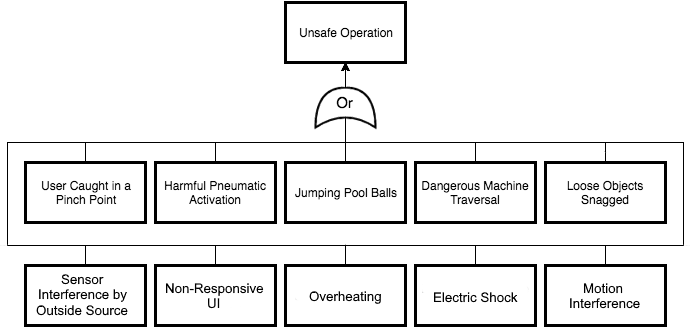
\includegraphics[width=0.9\textwidth]{SystemFTA.png}
\captionof{figure}{System FTA}
\label{fig:yRailFig}
\end{center}~\\[-8mm]
\subsection{User caught in a Pinch Point}
\textbf{Description}\\
When parts in a machine move in close proximity to one another, there is always a risk of harmful pinching. In this project, there are two locations where this may pose a notable risk: where the x-rails meet the arm base and where the y-rail meets the end-effector base.\\~\\
\textbf{Plans for Avoidance/Mitigation}\\
All pinch points will be clearly marked in order to signify the danger they present. Furthermore, emergency stop buttons will be located within reach of all pinch points in the case that a user finds themselves being harmed. This allows the damage to be minimized as much as possible in the case of a pinch. Also, a warning will be printed in a visible location on the system in order to warn users of this risk.\\~\\
The following diagram provides specific details for this hazard:\\
\begin{center}
	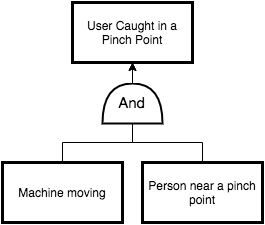
\includegraphics[width=0.35\textwidth]{PinchPointFTA.png}
\captionof{figure}{FTA for a user caught in a pinch point.}
\label{fig:yRailFig}
\end{center}

\newpage
\subsection{Harmful Pneumatic Activation}
\textbf{Description}\\
The pneumatic actuator will involve a very fast-moving component in order to strike the cue ball with sufficient force. If there is something in the way of the end-effector other than the cue ball such as the table, other parts of the machine, or a person, there is likely to be resulting damage.\\~\\
\textbf{Plans for Avoidance/Mitigation}\\
When the machine is about to take a shot a warning message or sound can be audibly played by the controller in order to alert the user to the upcoming movement. The machine will pause after this sound to allow the user time to stop the machine if there is an issue.\\~\\
The following diagram provides specific details for this hazard:\\
\begin{center}
	\includegraphics[width=0.35\textwidth]{PneumaticFTA.png}
\captionof{figure}{FTA for harmful pneumatic activation.}
\label{fig:yRailFig}
\end{center}

\newpage
\subsection{Jumping Pool Balls}
\textbf{Description}\\
Pool balls have a tendency to jump off the table if struck in a certain way. If the ball bounces off of the table, there is potential for damage to the machine, the surrounding environment, or a person.\\~\\
\textbf{Plans for Avoidance/Mitigation}\\
The end-effector will be designed in such a way that even when striking at its maximum force, the pool balls will never lose contact with the table. However, the user will still be playing on the table and might jump the balls. There is not much able to be done in terms of protecting other people or the surrounding environment unfortunately but the machine itself will be made in such a way that it is durable in areas where a jumping ball will be likely to hit it.\\~\\
The following diagram provides specific details for this hazard:
\begin{center}
	\includegraphics[width=0.9\textwidth]{JumpingBallsFTA.png}
\captionof{figure}{FTA for jumping pool balls.}
\label{fig:yRailFig}
\end{center}

\newpage
\subsection{Dangerous Machine Traversal}
\textbf{Description}\\
While the machine is traversing, anything in the way may be at risk. For example, depending on the speed, there could be damage due to impact. Another less severe example could involve knocking off items on the edges of the table.\\~\\
\textbf{Plans for Avoidance/Mitigation}\\
In order to avoid high speed impacts, the controller will simply not permit motion faster than a certain, safe speed. In terms of the knocking of items off the table, a warning will be printed in a visible location on the system in order to warn users of that risk. In addition, a warning message or sound can be audibly played by the controller in order to alert the user to upcoming movement. The machine will pause after this sound to allow the user time to stop the machine if there is an issue.\\~\\
The following diagram provides specific details for this hazard:
\begin{center}
	\includegraphics[width=0.9\textwidth]{DangerousTraversalFTA.png}
\captionof{figure}{FTA for dangerous machine traversal.}
\label{fig:yRailFig}
\end{center}

\newpage
\subsection{Loose Objects Snagged}
\textbf{Description}\\
At various locations -- namely the pinch points listed earlier as well as the rotational motor on the end-effector base and the belts on the x- and y-rails -- loose clothing, jewellery or long hair may be caught and pulled in. If these objects are attached to a person, this can lead to strangulation or being pulled into dangerous areas of the machine.\\~\\
\textbf{Plans for Avoidance/Mitigation}\\
For this hazard, there in not much to be done in terms of design to prevent the machine from snagging loose objects. However, a warning will be printed in a visible location on the system in order to warn users of this risk.\\~\\
The following diagram provides specific details for this hazard:
\begin{center}
	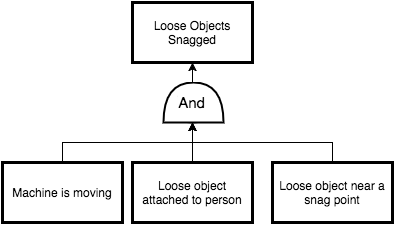
\includegraphics[width=0.5\textwidth]{LooseObjectFTA.png}
\captionof{figure}{FTA for loose objects being snagged.}
\label{fig:yRailFig}
\end{center}

\end{document}

